Literature review notes go here. \pt{This more technical stuff should go into a chapter before multi-agent communication. It can be framed as background and approaches to image captioning which are traditional in the sense that they are supervised. The transition to multi-agent communication could be task-specific or -conditional communication about visual environment which is a critically functional part of human communication. Chapter AFTER multi-agents should be language drift (jacob, lewis, andreas, 2021: multitasking inhibits drift ).}

\section{Introduction}

Make a table of definitions.

Sender / sepaker, receiver / listener, agents, message, distractor target. Image vectore representations extracted by a CNN / visual module = image features, backprop with ref. Reinforcement Learning = RL.
Do I need a more general section on like NNs, img captioning etc?

Maybe some RL stuff about the transitions, the stationary distribution etc?


\section{Image Captioning}
Producing sensible and informative captions for images has been a task that has received increasing attention in machine learning research over the last years. Importantly, in this domain, producing image captions in general is the only task of the developed applications; that is, the captions are not supposed to target any particular actionable goal other than producing captions close to the human examples seen during training---they are \textit{task-unconditional}. \pt{Point is clear, but sharpen the actual formulation. } From a machine learning perspective, the prerequisite for making image captions task-conditional would be the availability of supervised data from such a task. \pt{As discussed in the introduction, this motivates the choice of the multi-agent framework. Include and sharpen.} Nonetheless, technical advances developed in this domain provide the basis for agents employed in multi-agent settings; therefore, this section reviews selected work on image captioning in the computer vision and machine learning domain. The review focuses on more recent \textit{deep} models for iamge captioning \parencite{lecun2015deep}; for a review of earlier work, see, e.g., \pt{TBD}.

One of the first end-to-end deep neural architecture was developed by \cite{vinyals2015show}: the image captioner uses a CNN-based image feature extractor in order to extract vector representations from raw images, which are fed into an LSTM-based recurrent \textit{decoder} module, trained end-to-end to maximize the likelihood $\theta^* = argmax_{x} \sum_{(I, S)} log\; p(S \mid I; \theta)$ of example image descriptions $S$, given the image vector $I$ and the network parameters $\theta$. The descriptions are vectorized by a trainable embedding layer through which they are passed before being passed through the LSTM. \pt{Figure XX exemplifies the proposed training pipeline and the LSTM cell architecture.} The hidden size od the LSTM is 512, and it is trained using the so-called teacher forcing mode \pt{see below for details, ref}. The minimized loss is the sum of negative log likelihoods of the target words at each time step. Only the last layer of the CNN which is initialized with weights from a model pretrained on ImageNet is trainable. Furthermore, dropout layers and ensebling of the model (i.e., predictions from several models are combined to produce the reported results). The authors use beam search as the decoding strategy during inference and achieve a BLEU-4 score of 27.2 on the MS COCO test set (see section below \pt{ref} for details on the metrics), next to comparably high results on other datasets. 
This architecture is closely related to the architecture of the sender agent in the present experiments. \pt{CHECK: \cite{donahue2015long} propose a very similar approach.}

Another image captioning system was developed by \cite{karpathy2015deep}...: Check relation to Karpathy and Li 2014
\begin{itemize}
	\item CNN extracting regions: A Region CNN, pretrained on ImageNet and finetuned on 200 classes from ImageNet Detection Challenge, top 19 detected regions + whole image are kept and embedded intp 4096 dimensional space
	\item BRNN over captions, to address isue of dependencies etc when embedding words into visual space, using 300-dimensional word2vec embeddings. 
	\item compute alignment between them, predict captions based on inferred alignment through new Multimodal RNN architecture
	\item basic assumption: sentences are weak labels, which corespond to some unknown location in the image
	\item mention previous work where sentence templates are filled based on image content -- important for 3Dshapes experiment
	\item bidirectional recurrent net used to compute word representations, novel objective when learning alignment
	\item new objective: image-sentence score: dot product as single best alignment of a word to one image region, with margin maximization between align image-sentence pairs vs non-aligned ones
	\item goal: align text snippets, not only single words, to bounding boxes. This is achieved by treating the true alignment as a Markov Random Field, such that interactions between neighbouring words encourage alignment to the sam region.
	\item Multimpdal RNN: takes image pixels and a sequence of input vectors as input, where the image embedding is input as an additional bias at timestep 1. Hidden layer size is 512. The hidden layers are initialized with 0. They provide other important optimization details.
	\item They preprocess the sentences to lower-case, discarding non-alphanumeric characters. Importantly, they only keep words with frequency at least 5, resulting in 8791 words for 123000 MS COCO images. 
	\item the critical novelty is in the max margin loss which integrates the alignment score, which is used to train the BRNN
	\item ranking comparison on MS COCO reported -- check if I'll be able to compare to their performance.
	\item unclear how they train the MultimodelRNN on the alignment input -- they actually take the predicted labels for given bounding boxes from step before. For some reason, the annotators were asked to draw the bounding boxes, as opposed to receiving the ones proposed by the model.
\end{itemize}

\cite{xu2015show} propose a system where the image features are extracted using attention, computed on annotation vectors representing parts of the image. They compare stochastic attention to deterministic attention. The former is equivalente to the reinforce learning rule whereby the reward for the attention is proportional to the log likelihood of the target sentence. The latter is computed as a soft attention weight for the annotation vectors. This attention mechanism is diferentiable and, therefore, trainable end-to-end with back-propagation. The image location representation vectors were extracted using the VGGNet. For the experiment on MS COCO, they use a vocabulary size of 10.000; reported results are achieved with single models. The soft attention architecture allows to improve the test METEOR score on MS COCO by 0.02, while the hard attention does not yield an improvement, compared to \cite{vinyals2015show} (see Table \ref{tab_coco_metrics_ref}.

While the hitherto described systems consist of separate components used for representing the image and language parts, respectively, a different stream of work proposes, or, \textit{joint multimodal} representations of images and captions. \cite{kiros2014unifying} learn a joint image-caption embedding space, using LSTMs for encoding the captions. Image representations extracted via a CNN are projected into the LSTM hidden states to create the multimodal embeddings. Themultimodal embeddings are trained by maximizing cosine similarity between the image embedding and LSTM hidden state for the target image-caption pair, while minimizing the similarity to distractors. These multimodal embeddings are passed to a decoder module of various architectures which is then tested on image-sentence ranking and image captioning tasks. They show that multimodal embeddings outperforms object-detection based models, indicating that these LSTM embeddings develop meaningful description representations. \pt{double check last point}

Guided by the idea of creating combined representations, the most recent architectural innovation in this domain applies transformer layers for creating unified vision-language representations, ommiting the use of separate CNNs and RNNs \parencite{vaswani2017attention, zhou2019unified}. This work is also motivated by advances achieved with pretrained language models, such that a growing body of work develops multimodal language models. \pt{improve}
Originally, VLP \pt{check full introduction} architectures were developed in the computer vision domain for image understanding tasks like visual question answering or image classification \parencite{zhou2019unified}. \pt{check if VLP is coined in this paper or used before already as well} Crucially, the model is pretrained on image region embeddings combined with caption word embeddings in a transformer layer. Such pretraining is shown to be more effective on downstream tasks like image captioning after finetuning compared to non-pretrained architectures (see Table \ref{tab_coco_metrics_ref}, reported scores outperforming other models). 
% so-called \textit{transformers} for this task. Transformers have been first applied to an image processing task by \cite{dosovitskiy2020image}. More specifically, 
% Vision-Language-Pretraining (VLP) domain of tasks - matching images to texts, trained with "masked language modeling objective on images and their aligned descriptions ".  

Introduction of multimodal representation based models and more advanced architecture networks as agents in multi-agent communication settings relying on visual input is an interesting direction for future work. 

\subsection{Model Pretraining}

In this section, different approaches for training recurrent models which are predicting sequences, like the image captioning model is predicting a caption given the image, are discussed. In the context of multi-agent reference game experiments discussed in this thesis, this step can be seen as speaker agent pretraining.

It is assumed that the target task for the model is predicting the next token of a sequence, given the preceding tokens; this task is at the core of various applications like neural machine translation, image caption generation, text sumamrization and others \pt{REF}. This task is usually modelled by recurrent neural networks \pt{ref}. The challenge when training recurrent neural network models which are predicting sequences at inference time by replicating the inference time scenario, i.e., by conditioning the next token on the output of the model itself at the previous timestep, is slow convergence of the training, its instability and potentially poor generation skills \pt{Maybe just the ML book, but more specifics on the issues are needed. Original source: https://machinelearningmastery.com/teacher-forcing-for-recurrent-neural-networks/ }. The main approach that has been proposed in order to mitigate these issues is \textit{teacher forcing}, with several extensions to: \textit{search over candidate output sequences}, \textit{curriculum learning} and \textit{professor forcing} \parencite{goodfellow2016deep, williams1989algorithm}.

When using curriculum learning, at each step the source of input, i.e., whether it is the ground truth or the output of the previous timestep, to the next time step is chosen randomly \parencite{bengio2015scheduled}. This curriculum anneals over time, starting at teacher forced learning only (i.e., al inputs are ground truth tokens) at gradually transitioning to using predicted inputs. Inverse sigmoid decay schedule for the probability of the coin flip determining where the next input token come from was shown to yield best results on the MS COCO image captioning task.

When using professor forcing, the discrepancey between the training and inference performance is addressed by minimizing the discrepancy between the teacher forced and auto-regressive sampling behaviour, i.e., by making the distribution over sequences during training maximally similar to the target distribution \parencite{lamb2016professor}. This is achieved by training the model as a Generative Adversarial Network (GAN). More specifically, a second recurrent network---a biderectional RNN---  is introduced additionally to the RNN generating the captions. Due to the additional overhead for training an image captioner with this approach, exploring the effects of such pretraining on the downstream reference game is left for future work.

For conducting the experiments in this thesis, speakers pretrained with different following approaches are considered: pure teacher forcing pretraining, constant 0.5 rate teacher forcing, linear adaptive teacher forcing, scheduled sampling (with pure decoding, k = 30, ?) na topk sampling with a tenmperature of 2 (replicating \cite{lazaridou2020multi}). \pt{For details of selecting the final pretrained speaker, see XY. }

\subsection{Evaluation Metrics}
An important yet non-trivial aspect of developing image captioning systems is their evaluation. Image captioning has been considered difficult to evaluate because for a given input image, several output captions might be equally suitable \pt{REF. Maybe example}. Therefore, usually a suite of evaluation metrics is used for evaluation. This work employs the merics proposed for the MS COCO dataset \parencite{chen2015microsoft}: BLEU-$n$, ROUGE, METEOR and CIDEr scores. In this section, conceptual aspects of these metrics applied to image captioning are introduced; for formal derivations, see, e. g., \cite{chen2015microsoft}.\footnote{The implementation of these metrics in Python provided by \url{https://github.com/daqingliu/coco-caption} is used in the present experiments.}

The BLEU-$n$ score evaluates the co-occurence on $n$-grams between generated and reference sequences \parencite{papineni2002bleu}. More precisely, the corpus-level $n$-gram precision is computed (fraction of relevant n-grams in the generated n-grams). That is, all reference captions as considered as a corpus, and the overall score is computed as a weighted geometric mean over all $n$-grams. However, BLEU favors short sentences and has been shown to be a poor metric for single sentence comparisons, especially when considering longer $n$-grams. \pt{check if rouge is needed---only is any reference values can be found.}

%The ROUGE metric was developed for text summarization evaluation and has three variations: ROUGE$_N$, ROUGE$_L$ and ROUGE$_S$. ROUGE$_N$ computes $n$-gram recall over all ground truth captions given the generated one (=fraction of found ground truth n-grams); ROUGE$_L$ is the $F$-score computed over the lengths of so-called \textit{Longest Common Subsequence} (i.e., an n-gram where other words may occur in between). Finally, ROUGE$_S$ is computed as $F$-score over counts of skip bigrams (i.e., bigrams where k words may occur in between).  Generally, the ROUGE scores are somewhat better at capture longer-range sentence structure preservation.

METEOR is computed by generating alignments between target and generated captions \parencite{banerjee2005meteor}. The alignments are based on both matching exact tokens and matching WordNet synonyms, stems and other generalizations. Then, the harmonic mean between the precision and recall over the best target-generated caption pairs, and the final score includes a penalty for quality of the found alignments. METEOR is computed as a corpus level metrics, as well, meaning that all target captions ar aggregated.
 
Finally, CIDEr is a native image captions evaluation metric \parencite{vedantam2015cider}. It is computed as a weighted TF-IDF for each $n$-gram occurring in the ground truth captions for the set of all images. Intuitively, the weighting provides a trade-off between common and distinctive n-grams. These weights are then combined into vectors for each n-gram of length $n$, based on which average cosine similarity between vectors for ground truth and generated captions is computed. The final CIDEr score is obtained as the average over the single n-gram similarities. In order to increase the similarity of metric results to human intuitions, further modifications including caption length-based gaussian penalties are included. Intuitively, CIDEr captures the similarity in distinctness or saliency of the generated and ground truth captions.

\pt{Recall based metrics usually reported.. seem to be related to the metrics including soome notion of recall?}

Since these metrics can only be computed in the presence of ground truth image captions, they are first and foremost applied in experiments on the MS COCO dataset, as experiments on the 3Dshapes dataset are based on self-generated ``ground truth'' captions and no reference values exist for this dataset.
Previous work on captioning the MS COCO datase discussed in this section provides a baseline for evaluating the quality of captions produced in this work. Table \ref{tab_coco_metrics_ref} provides and overview of scores achieved with extant systems.

\begin{table}[]
	\begin{tabular}{|l|l|l|l|l|l|l|l|}
		\hline
		Model                               & BLEU-1 & BLEU-2 & BLEU-3 & BLEU-4 & METEOR & CIDEr \\ \hline
		\cite{bengio2015scheduled}        & -      & -      & -      & 0.323   & 0.254  & 0.987 \\ \hline
		\cite{vinyals2015show}  & -      & -      & -      & 0.277    & 0.237  & 0.855 \\ \hline
		\cite{xu2015show} & 0.718  & 0.504  & 0.357  & 0.250     & 0.239  & -     \\ \hline
		\cite{karpathy2015deep}          & 0.625  & 0.450  & 0.321  & 0.230   & 0.195  & 0.660 \\ \hline
		\cite{zhou2019unified}          & -  & -  & -  & 0.365   & 0.284  & 1.179 \pt{?} \\ \hline
	\end{tabular}
\caption{\label{tab_coco_metrics_ref}The table shows metrics for the quality of captions generated on respective test sets of the MS COCO dataset. Best results reported in each paper are included.}
\end{table}

\section{Reinforcement Learning}

\subsection{Introduction}
A natural choice for training artificial agents to complete certain tasks like communicative tasks is reinforcement learning, as ``Reinforcement learning is a computational approach to understanding and automating goal-directed learning and decision-making'' (s.15, \cite{sutton2018reinforcement}).

``The reinforcement learning problem is meant to be a straightforward framing of the problem of learning from interaction to achieve a goal. The learner and decision-maker is called the agent. [...] These interact continually, the agent selecting actions and the environment responding to those actions and presenting new situations to the agent.'' (p.53). A particular task is defined in terms of a complete definition of the environment, representing a particular instance of reinforcement learning (p. 54).

Therefore, reinforcement learning can be defined as learning the mapping from situations, represented as \textit{environments}, to optimal \textit{actions} that agent may choose in order to achieve the task goal, while maximizing the reward signal \parencite{sutton2018reinforcement}. Next to supervised and unsupervised learning, it represents one of three major learning paradigms in machine learning. 

\begin{figure}
	\centering
	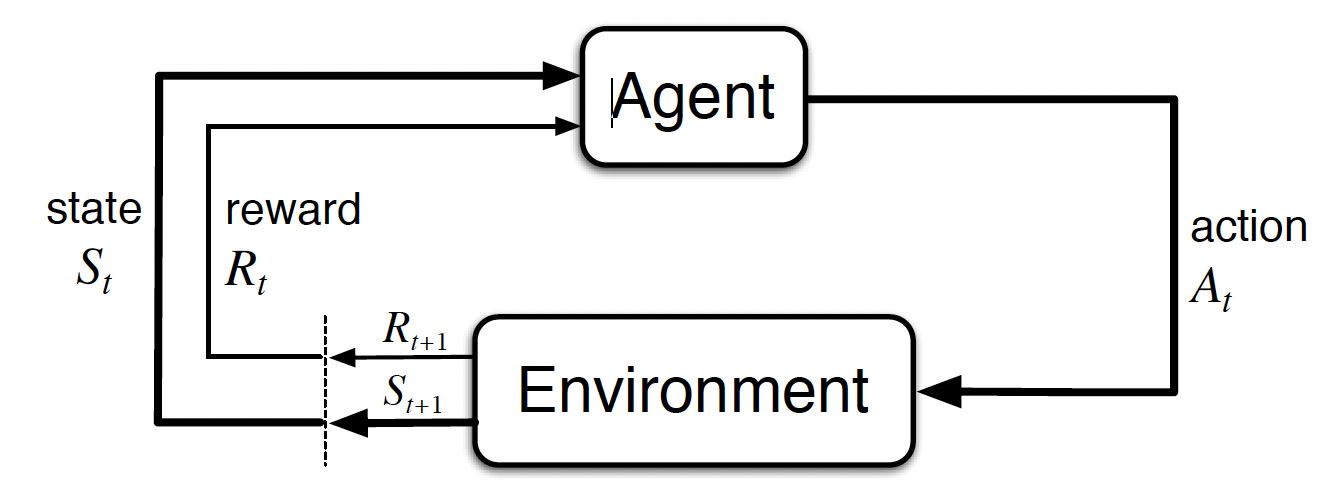
\includegraphics[width=0.8\linewidth]{images/rl_intro.png}
	\caption{Interaction the environment with the agent via states, actions and rewards \parencite{sutton2018reinforcement}.}
	\label{fig:rl}
\end{figure}

\pt{Definitions of: reward, environment, agents, actions, states, policy, value function, if necessary, q-learning maybe. An optiional model of the environment may also exist. }
\begin{itemize}
	\item agent: learner and decision maker in the interaction who tries to achieve a goal for a certain task.
	\item the setting in which the agent's interactions are situates, everything outside of the agent itself is the \textit{environment}.
	\item policy: the agent's learned mapping from environment states to actions within the environment 
	\item reward signal: ``defines the goal in a reinforcement learning problem'' (p. 7, \cite{sutton2018reinforcement}) which is made up from single \textit{rewards} the agent receives at each timestep of the decision process. Improtantly, the agents' goal is to maximize the sumn of the rewards over the task completion.
	\item value function: the expected total reward for agents starting the actions at the given state. These are adapted and reestimated based on observed action and reward sequences of the agents over their lifetime. 
\end{itemize}

Situations modelled by reinforcement learning are decision making sequences; such sequences are typically and straightforwardly formalized as Markov decision processes (MDPs), framing the problem of interactively learning to achieve a goal from interaction (p. 47). Here it is assumed that the interaction takes place over discrete timesteps $t = 0, 1,2 ...$. At each step $t$, the state $S_t \in S$ in which the agent is in can be considered as her current representation of the environment, where $S$ is the set of all possible states. Given the state, the agent selects an action $A_t \in A(s)$, where $A(s)$ denotes the set of all actions available in state at time $t$. At the next timestep the agent receives a reward $R_{t+1} \in R$ for the action $A_t$. These iterations can be formalized as finite MDPs if they consist of an $A, S$ and $R$ with a finite number of elements. In this case, the probability $p$ for a particular state $s'$ and reward $r'$ to occur at time $t$ is conditional on the previous state and action. A typical assumption made in the RL literature applied to multi-agent communication is that the states have the \textit{Markov property}, i.e., that they encode information from all previous interaction steps. Given $p$, one can compute state transition probabilities (i.e., probabilities for getting into a particular state given previous cisited states), and most critically, the expected rewards for given state and action combinations. The latter is especially important in order to estimate the return $G_t$ and thus, formally represent the objective of learning, namely maximizing the return. In present work, the following simple definition of $G_t$ is assumed: 
$$G_t = R_{t+1} + R_{t+2} + ... + R_T$$ where $T$ is the final step of the action sequence. This sequence as a natural iteration of interactions is also called \textit{episodes}.  Different return formalizations, e.g., using expected discounted returns is popular in other domain, but cannot really be applied in the present reference game since the environment (i.e., the reference game) only provides one reward per entire episode (i.e., entire message generation). 

Another critical part of RL algorithms is the value function, describing how valuable it is with respect to the expected return for an agent to be in a given state. Since these values depend on the taken actions, the last critical component is the policy. ``A policy is a mapping from states to probabilities'' of taking avalibale action: $\pi(a | s)$ the describes the probability that the agents choses the actiona inthe state s. The central problem of RL is then the estimation of an optimal policy, yielding a maximal reward. The following section reqviews different methods for estimating the policy, especially fpcusing on methods applicable to \textit{deep RL}, i.e., RL with deep neural network agents \parencite{lecun2015deep}.

Terminal state = state at the end of each episode.
Action-value function? value function? necessary?

% Concrete specification and notation of actions, rewards, states and policy.

(Discounted) rewards.

Value functions and optimal policies (up to p. 95).

Transition to deep reinforcement learning \parencite{lecun2015deep}.

\subsection{Deep Reinforcement Learning Methods}

Deep Q-learning. 

The so-called Actor-Critic methods consist of the policy acting as the actor from which the actions are sampled, and a critic, which is usually represented by the action value function \pt{def doublec hcek and refine}. The goal hereby is to estimate whether the chosen action improves the current state.  

\pt{Policy-gradient method reinforce \parencite{williams1992simple, sutton2018reinforcement}. Mean baseline. } A particular framework, the so-called \textit{policy-gradient methods} for estimating the policy focus on improving the parameters of the policy, while taking advantage of observation made about the agent's individual interactions with the environment (p. 10). More specifically, this approach provides a solution to the issue of computational intractability of analytically solving for an optimal policy (p. 80) and instead focuses on the agent's experience simulated from the environmant.  



\pt{Add machine details in the expts section}